\section{Cartographie fonctionnelle cible}
\label{sec:fonctionnel}

\subsection{Plan d'occupation des sols}
La cartographie fonctionnelle (figure~\ref{fig:fonctionnel}) décrit ce que le système cible doit savoir faire, indépendamment des logiciels qui le feront. Elle est organisée en six zones, conformément aux pratiques d'urbanisation \cite{longepe2009}~: une zone d'\emph{échange} regroupant les canaux, une zone \emph{opérationnelle} portant le cœur du métier, une zone de \emph{support}, une zone de \emph{pilotage et d'IA}, une zone de \emph{ressources} et une zone de \emph{référentiels et d'échanges} avec les systèmes externes. Chaque bloc porte son statut~: \tagE~existant, \tagV~à faire évoluer, \tagN~nouveau.

\begin{figure*}[t]
\centering
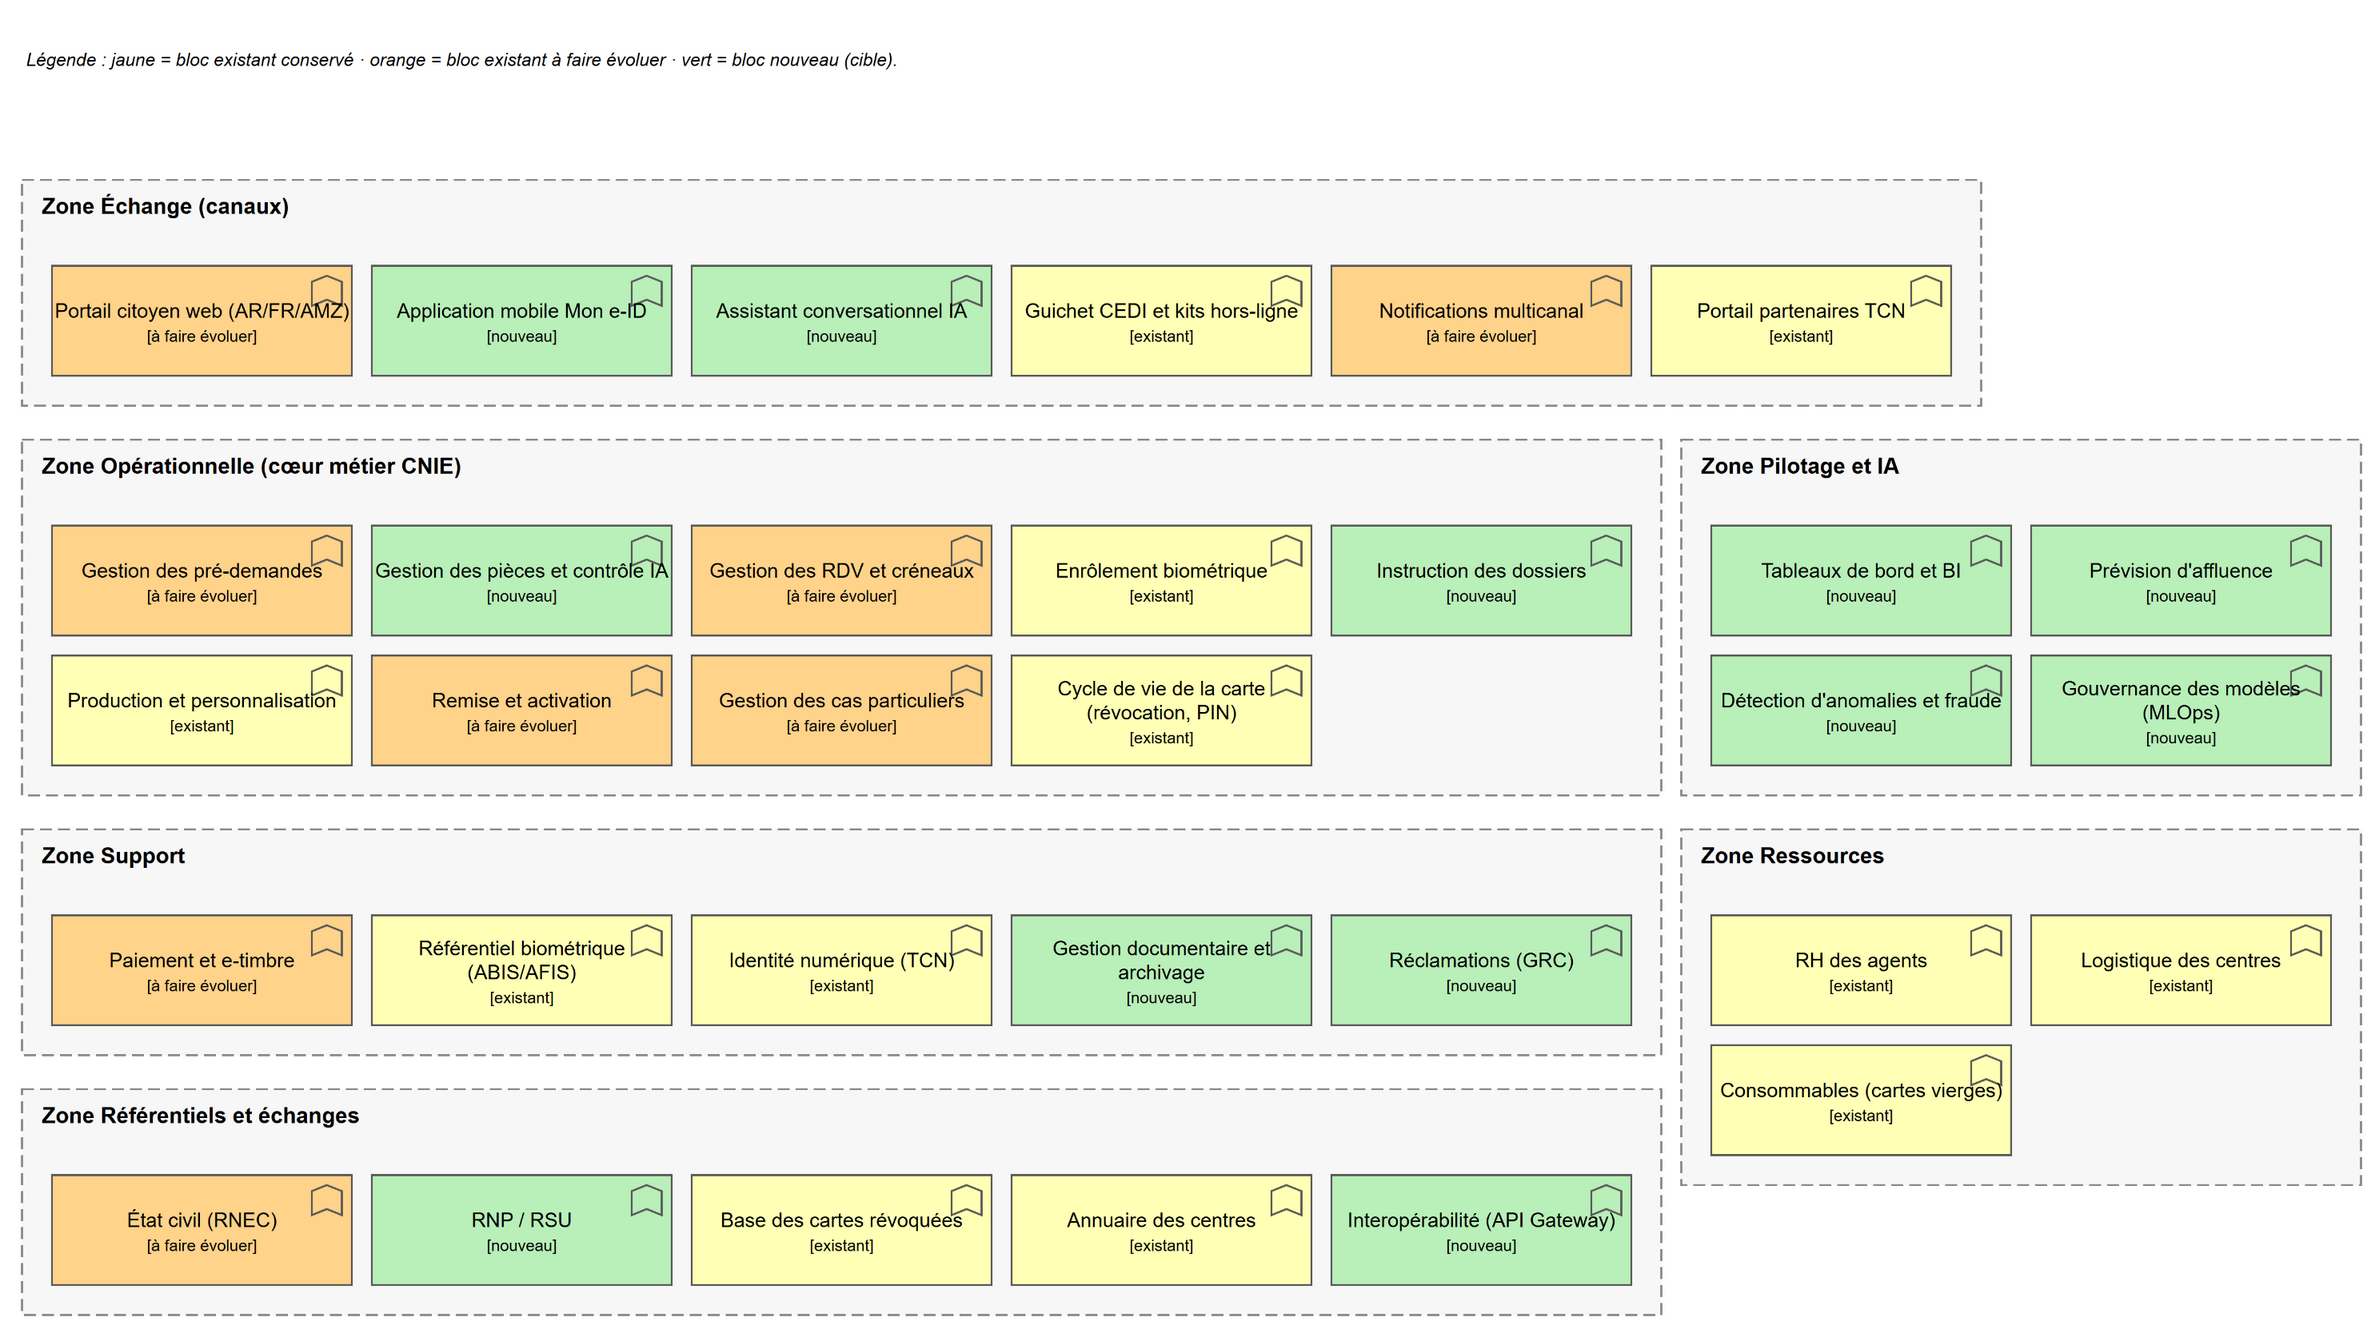
\includegraphics[width=0.98\textwidth]{archimate/V3_fonctionnel.png}
\caption{Plan d'occupation des sols fonctionnel cible~: 32 blocs répartis en six zones, avec mise en évidence des blocs existants, à faire évoluer et nouveaux.}
\label{fig:fonctionnel}
\end{figure*}

\subsection{Lecture zone par zone}
\paragraph{Zone Échange} Le portail web est conservé mais refondu (multilingue, accessible, adaptatif), tandis que deux canaux nouveaux apparaissent~: l'application mobile «~Mon e-ID~», qui fusionne la carte numérique et le suivi des demandes, et l'assistant conversationnel (IA-1). Le guichet des CEDI et les kits hors-ligne de la plateforme Tiers de Confiance restent indispensables pour l'inclusion. Les notifications deviennent multicanal (SMS, e-mail, notification mobile).

\paragraph{Zone Opérationnelle} Deux blocs nouveaux concentrent la valeur de la cible~: la \emph{gestion des pièces et contrôle IA} (IA-2) et l'\emph{instruction des dossiers}, qui outille le nouvel acteur back-office. La gestion des pré-demandes, des rendez-vous, de la remise et des cas particuliers évolue pour s'intégrer au moteur de processus. L'enrôlement biométrique, la production et le cycle de vie de la carte sont conservés tels quels, car ils reposent sur des équipements et des procédures de sécurité éprouvés.

\paragraph{Zone Support} Le paiement évolue vers une vérification en ligne de l'e-timbre. Le référentiel biométrique et l'identité numérique existent déjà. Deux fonctions nouvelles s'ajoutent~: la gestion documentaire avec archivage à valeur probante, rendue nécessaire par la dématérialisation des pièces, et la gestion des réclamations.

\paragraph{Zone Pilotage et IA} Entièrement nouvelle, elle regroupe les tableaux de bord, la prévision d'affluence (IA-4), la détection d'anomalies et de fraude (IA-5) et la gouvernance des modèles (suivi des performances, des biais et des versions), sans laquelle l'usage de l'IA dans un service régalien ne serait pas acceptable.

\paragraph{Zones Ressources et Référentiels} Les ressources humaines, logistiques et les consommables sont hors du périmètre de transformation. En revanche, la zone des référentiels s'ouvre~: l'accès à l'état civil devient automatisé, l'interconnexion au Registre National de la Population est préparée, et une fonction d'interopérabilité unique (passerelle d'API) encadre tous les échanges.

\subsection{Matrice de couverture}
Le tableau~\ref{tab:couverture} vérifie que chaque capacité stratégique est portée par au moins un bloc fonctionnel, et que chaque bloc nouveau se justifie par un objectif.

\begin{table}[h]
\caption{Couverture des capacités cibles par les blocs fonctionnels}
\label{tab:couverture}
\centering
\small
\begin{tabularx}{\columnwidth}{lX}
\toprule
\textbf{Capacité} & \textbf{Blocs fonctionnels contributeurs} \\
\midrule
Gestion des demandes de titre & Pré-demandes \tagV, pièces et contrôle IA \tagN, RDV \tagV, instruction \tagN, remise \tagV, cas particuliers \tagV \\
Enrôlement biométrique & Enrôlement \tagE, référentiel biométrique \tagE, guichet et kits \tagE \\
Identité numérique et authentification & Identité numérique TCN \tagE, app Mon e-ID \tagN, portail partenaires \tagE \\
Contrôle documentaire par IA & Pièces et contrôle IA \tagN, gestion documentaire \tagN, assistant \tagN \\
Pilotage prédictif & BI \tagN, prévision \tagN, anomalies \tagN, MLOps \tagN \\
\bottomrule
\end{tabularx}
\end{table}
